% Appendix E: Causal Validation Experiments

\section{Causal Validation Experiments}
\label{app:causal_validation_details}

% 本节提供正文 §3.1 三组因果实验的完整设置、层位扫描结果与失败案例。

\subsection{Activation Patching at FJC}
\label{app:subsec:activation_patching_fjc}

% 详细实验设置：task-matched sample 配对策略、patching 操作流程。
% 层位扫描：不同层的 answer-flip rate 曲线，展示 FJC 的因果特权性。
% 预期效果：读者可看到 FJC 层 flip rate 相对其他层的显著优势。

% TODO: 插入 patching 实验细节与层位扫描图

\subsection{Layer Skipping for Overprocessed}
\label{app:subsec:layer_skipping_overprocessed}

% 跳过 FJC 之后尾部层的具体操作与解码方式。
% Resolved vs. Overprocessed 上的效果对比，展示 outcome 特异性。
% 预期效果：证明 Overprocessed 确实是"先对后错"，跳过后期层可恢复。

% TODO: 插入 layer skipping 实验结果

\subsection{Late-Layer Hidden-State Sparsity in Overprocessed Samples}
\label{app:subsec:late_layer_sparsity_overprocessed}

As a descriptive complement to the layer-skipping intervention, we also examine whether Overprocessed samples exhibit a distinct late-layer representation geometry.
Using the full Qwen2.5-Coder-7B Computing dataset ($N=1800$), we aggregate two standard sparsity measures from the last-token hidden state at every layer: the Gini index and Hoyer sparsity.

\cref{fig:app:hidden_state_sparsity} shows that the two measures peak at different depths.
The Gini index rises earlier and reaches its maximum around the middle-to-late layers, whereas Hoyer sparsity stays relatively moderate until the final block and then spikes sharply near layer 26.
This temporal separation is consistent with a two-stage picture in which representations first become more concentrated and later undergo a stronger sparsification during the final decoding-relevant phase.

To test whether this late sparsification is specifically associated with degradation after internal success, we compare Overprocessed and non-Overprocessed valid samples at layers 24--27.
As shown in \cref{fig:app:hoyer_ot_vs_nonot}, Overprocessed samples have consistently higher Hoyer sparsity at all four late layers, with the largest gap at layer 26 where global Hoyer also peaks.
Because this analysis is observational rather than interventional, we do not treat sparsity as causal evidence.
Instead, we view it as a representation-level correlate of overprocessing: once a correct answer has become jointly available, the final degradation phase is accompanied by a measurable compression-like shift in hidden-state geometry.

\begin{figure*}[t]
\centering
\begin{subfigure}[t]{0.58\textwidth}
    \centering
    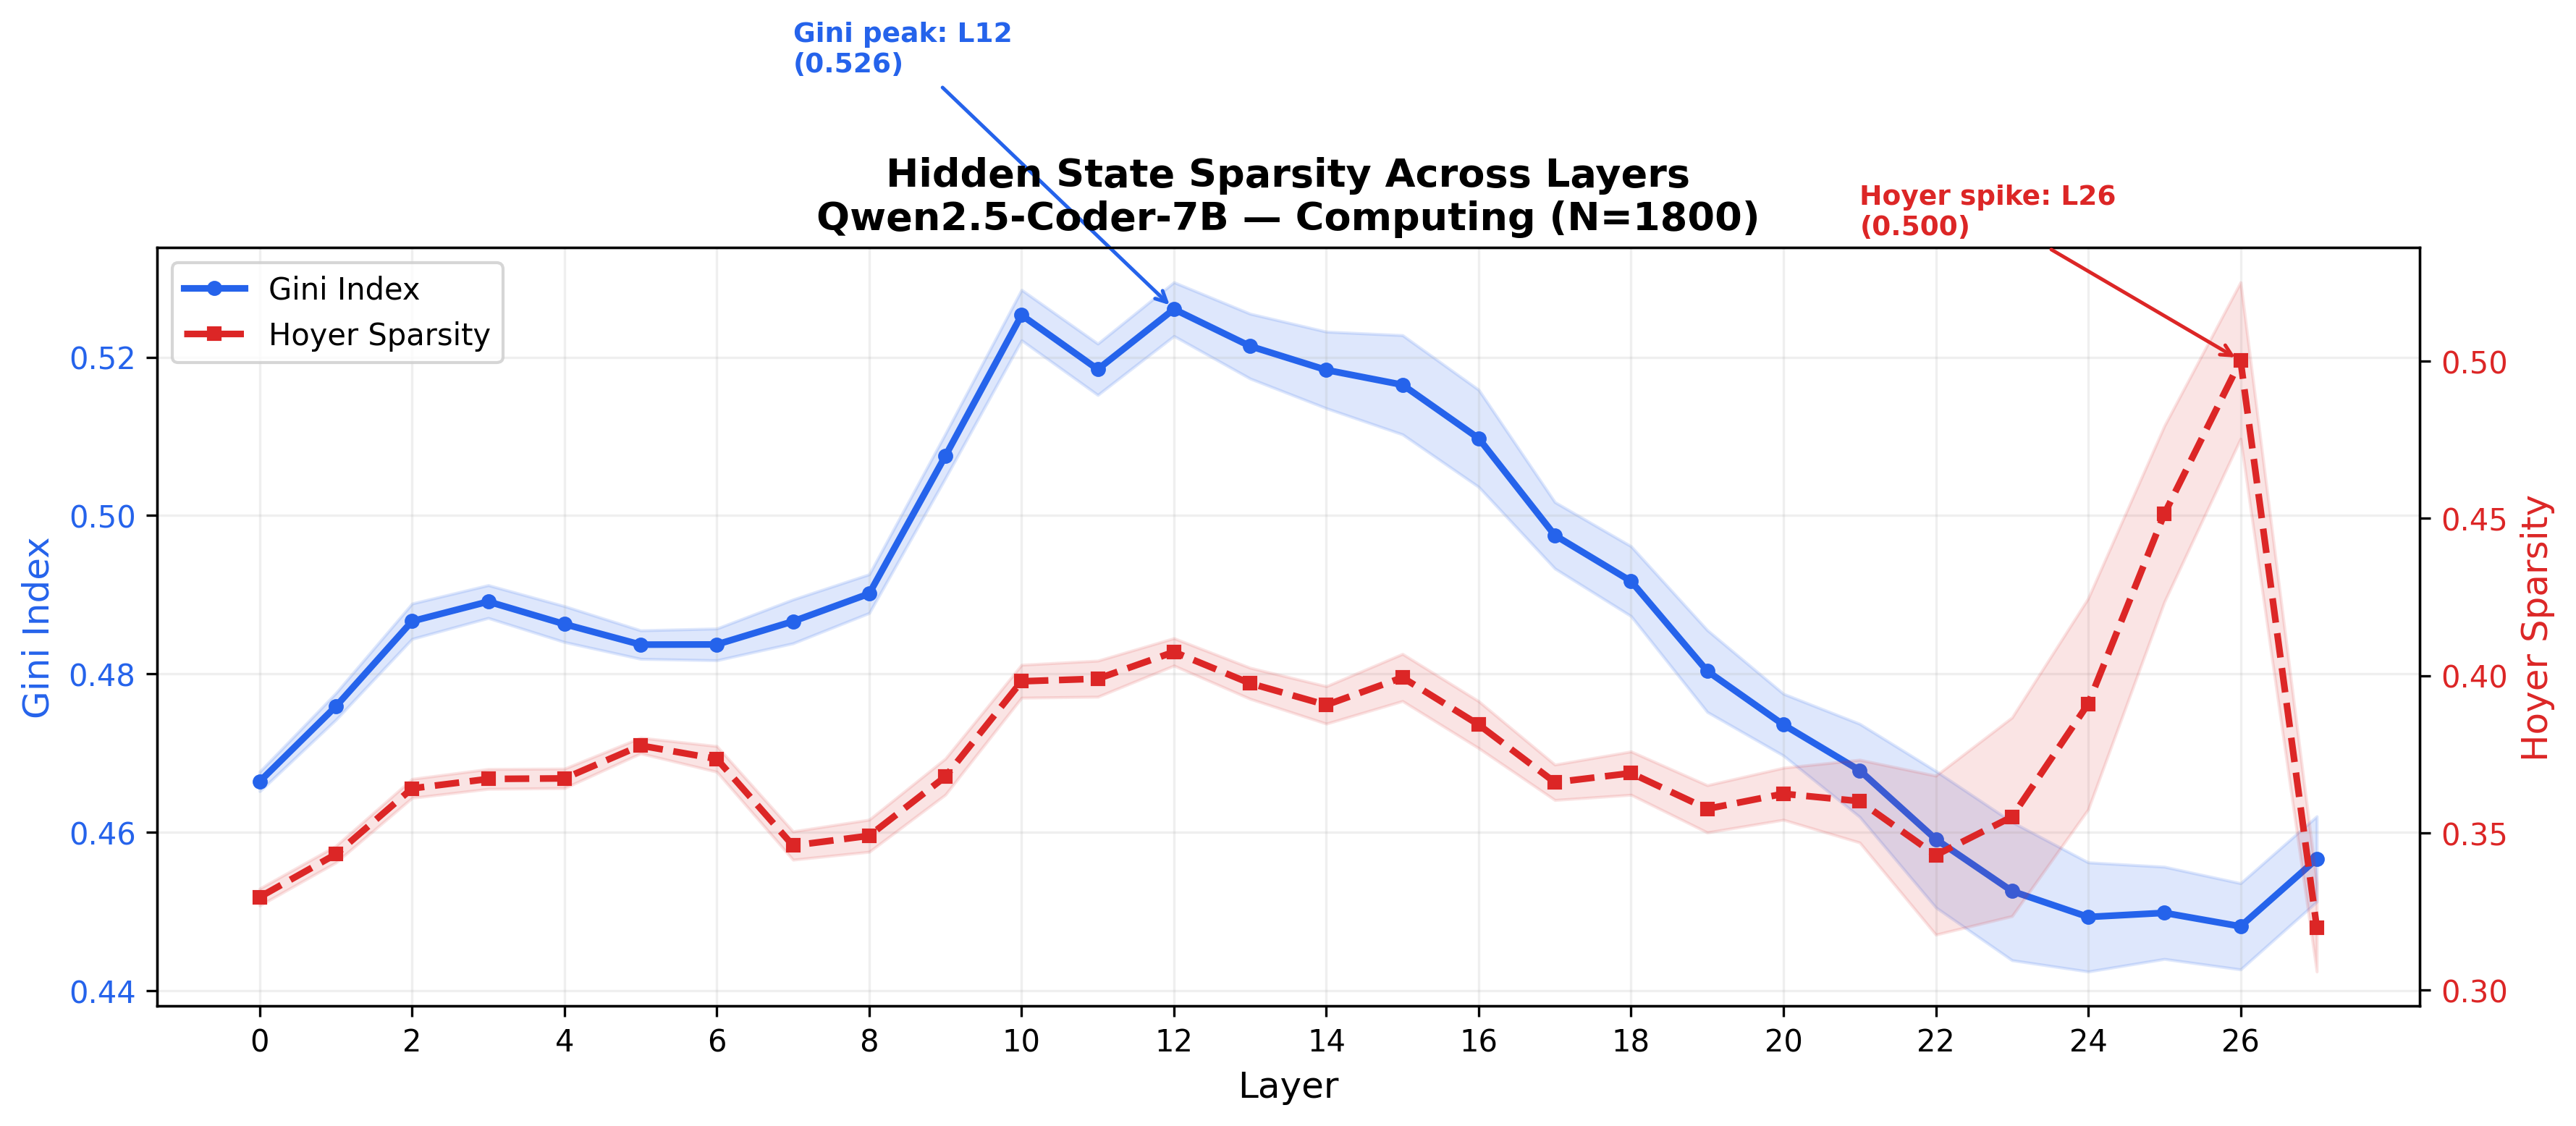
\includegraphics[width=\textwidth]{figures/appendix/causal_hidden_state_sparsity.png}
    \caption{Global layer-wise Gini and Hoyer curves on the full Qwen2.5-Coder-7B Computing set.}
    \label{fig:app:hidden_state_sparsity}
\end{subfigure}
\hfill
\begin{subfigure}[t]{0.38\textwidth}
    \centering
    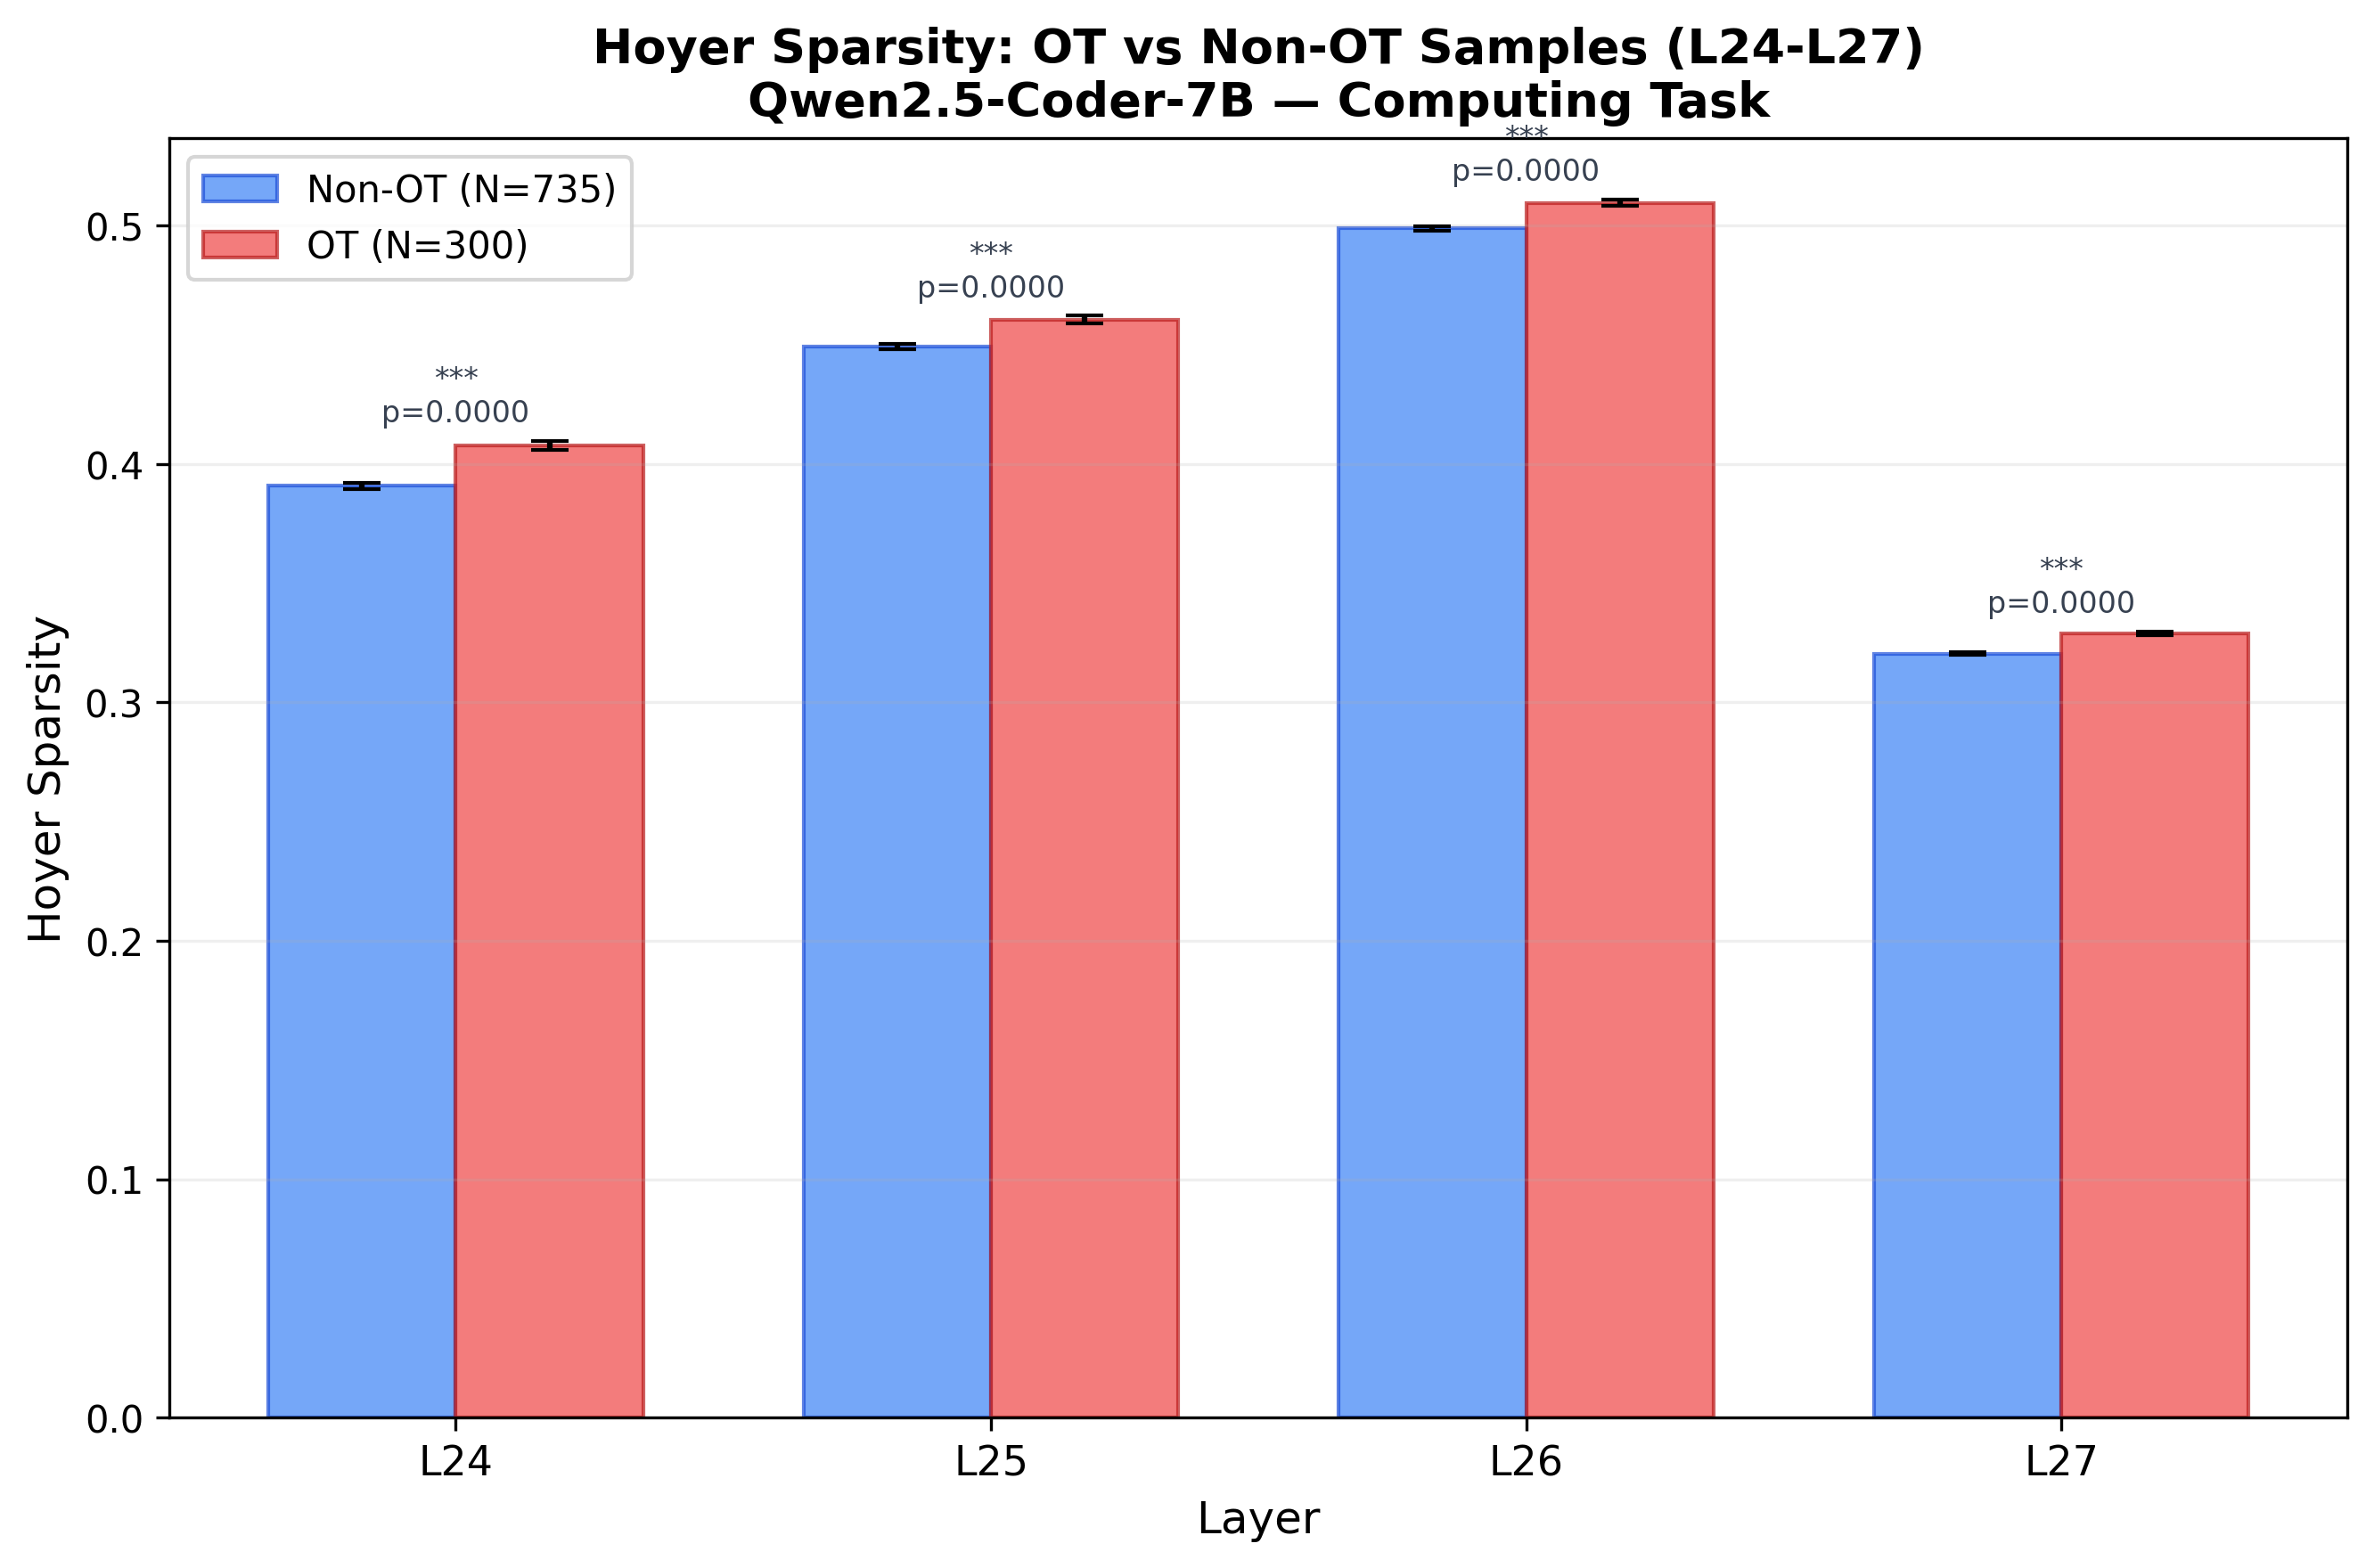
\includegraphics[width=\textwidth]{figures/appendix/causal_hoyer_ot_vs_nonot.png}
    \caption{Late-layer Hoyer sparsity for Overprocessed vs.\ non-Overprocessed valid samples.}
    \label{fig:app:hoyer_ot_vs_nonot}
\end{subfigure}
\caption{Late-layer hidden-state sparsity as a descriptive correlate of Overprocessed trajectories in the anchor setting (Qwen2.5-Coder-7B, Computing).}
\label{fig:app:overprocessed_sparsity}
\end{figure*}

\subsection{Re-injection for Unresolved}
\label{app:subsec:reinjection_unresolved}

% 重注入流程：如何将后期 hidden state 注入新的前向传播以提供额外有效深度。
% Rescue rate 计算与结果。
% 预期效果：证明 Unresolved 多数是"没算完"而非"根本不会"。

% TODO: 插入 re-injection 实验结果

\subsection{Failure Cases}
\label{app:subsec:causal_failure_cases}

% 三组因果实验中干预无效的典型案例分析。
% 预期效果：诚实地展示方法边界，增强可信度。

% TODO: 插入失败案例分析
